% called by main.tex
%
\chapter{Resultados}
\label{sec::capitulo4}
\section{Detección de distracción}
\subsection{Resultados de entrenamiento de modelos de aprendizaje profundo}
La Figura \ref{fig:CNNs} muestra los resultados de entrenamiento de distintas arquitecturas de aprendizaje profundo para la predicción de las categorías \textit{looking\_road} y \textit{not\_looking\_road}. Se muestran las métricas que se consideran relevantes para los resultados, siendo la precisión, sensibilidad, \textit{F1 score}, y AUC, valores los cuáles nos indican de manera descriptiva que tan bueno es el modelo para predecir de manera mas detallada. Los valores de \textit{F1 score} tienen un rango de 0.856 a 0.996, mostrando la variabilidad de las arquitecturas utilizadas para la experimentación, obteniendo así resultados deseados para el entrenamiento de modelos con una gama de modelos con distintas capacidades de predicción y diferentes niveles de consumo computacional. 

\begin{figure}[h!]
    \centering
    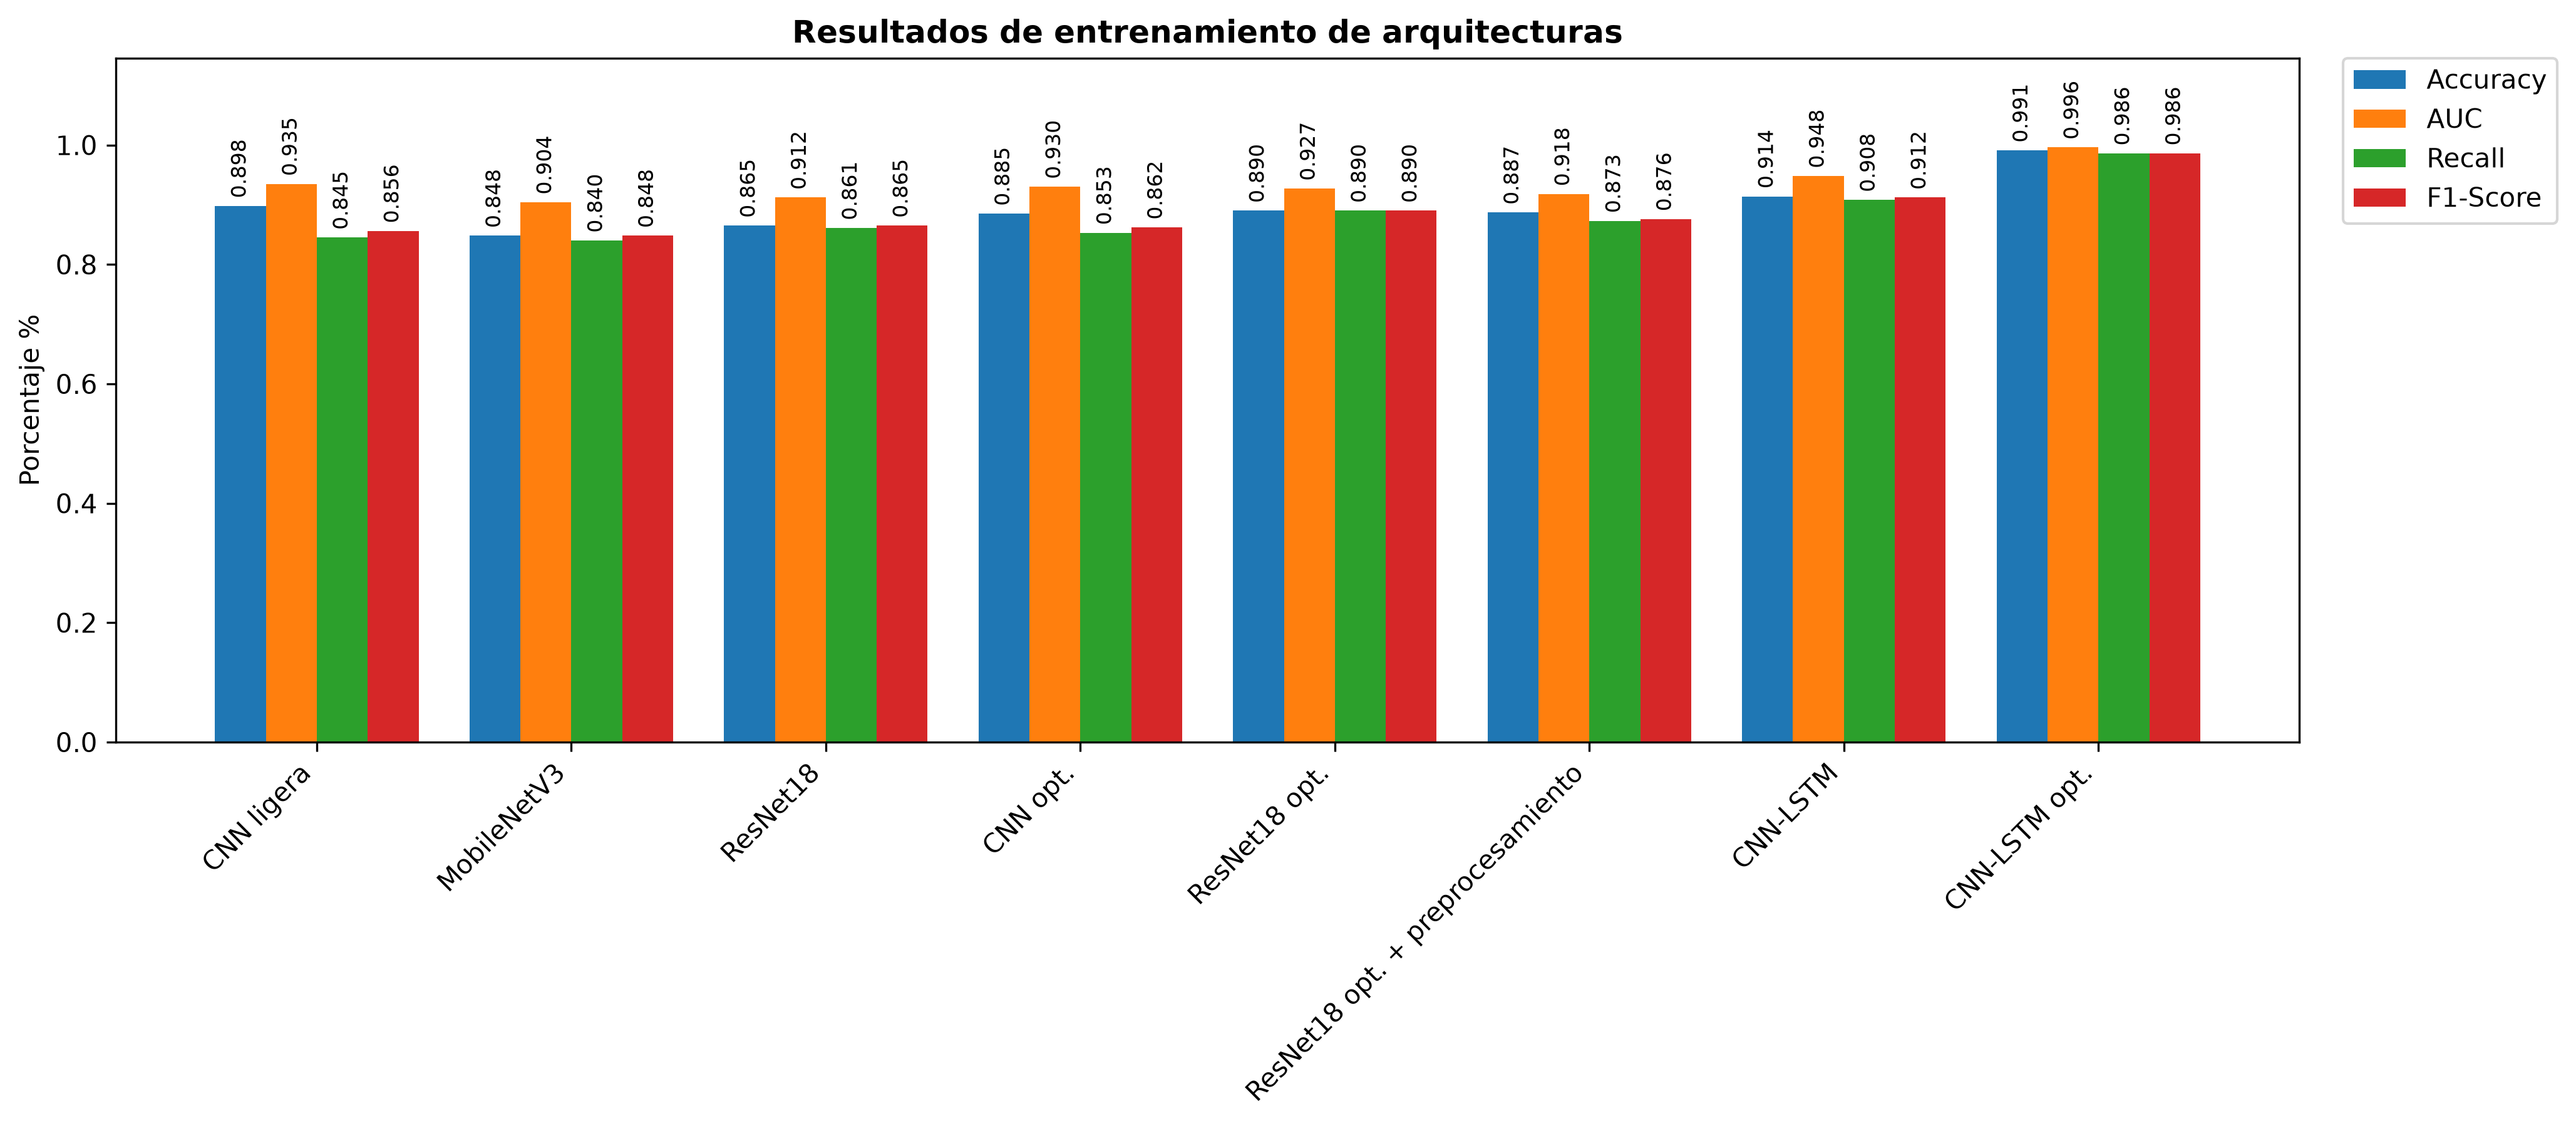
\includegraphics[width=1\linewidth]{figures/resultados_arquitecturas.png}
    \caption{Resultados de experimentación en entrenamiento de modelos de aprendizaje profundo}
    \label{fig:CNNs}
\end{figure}

\newpage %por ahora
\subsection{Rendimiento de algoritmos en tiempo real}


La Figura \ref{fig:lat} muestra los tiempos de inferencia promedio de cada uno de los modelos, tanto en una laptop con GPU como en la RapberryPi 5B, nuestro dispositivo objetivo a implementar en tiempo real. 
Podemos ver los comportamientos inicialmente esperados, con tiempos mucho menores en la laptop, debido a la capacidad computacional que esta ofrece. En ambos casos el menor tiempo de inferencia lo muestra LightGazeCNN, la CNN creada para esta investigación. 
Igualmente, en ambos casos la arquitectura con mayor tiempo de inferencia es la C-LSTM, esto debido a su complejidad al combinar una ResNet18 con dos capas LSTM. El tiempo de inferencia menor en la RaspberryPi 5B es de 11.8ms y el mayor de 82.4ms, mientras que en la laptop son de 3.4ms y 11.1ms, lo cuál muestra la importancia de tomar en cuenta el poder computacional que se tiene en el equipo utilizado. Igualmente, los FPS a los cuáles funcionan cada tarea son diferentes, teniendo en promedio 13 para la tarea de distracción, 18 para la tarea de somnolencia y 33.61 para la tarea de captura de imagen.  

\begin{figure}[h!]
    \centering
    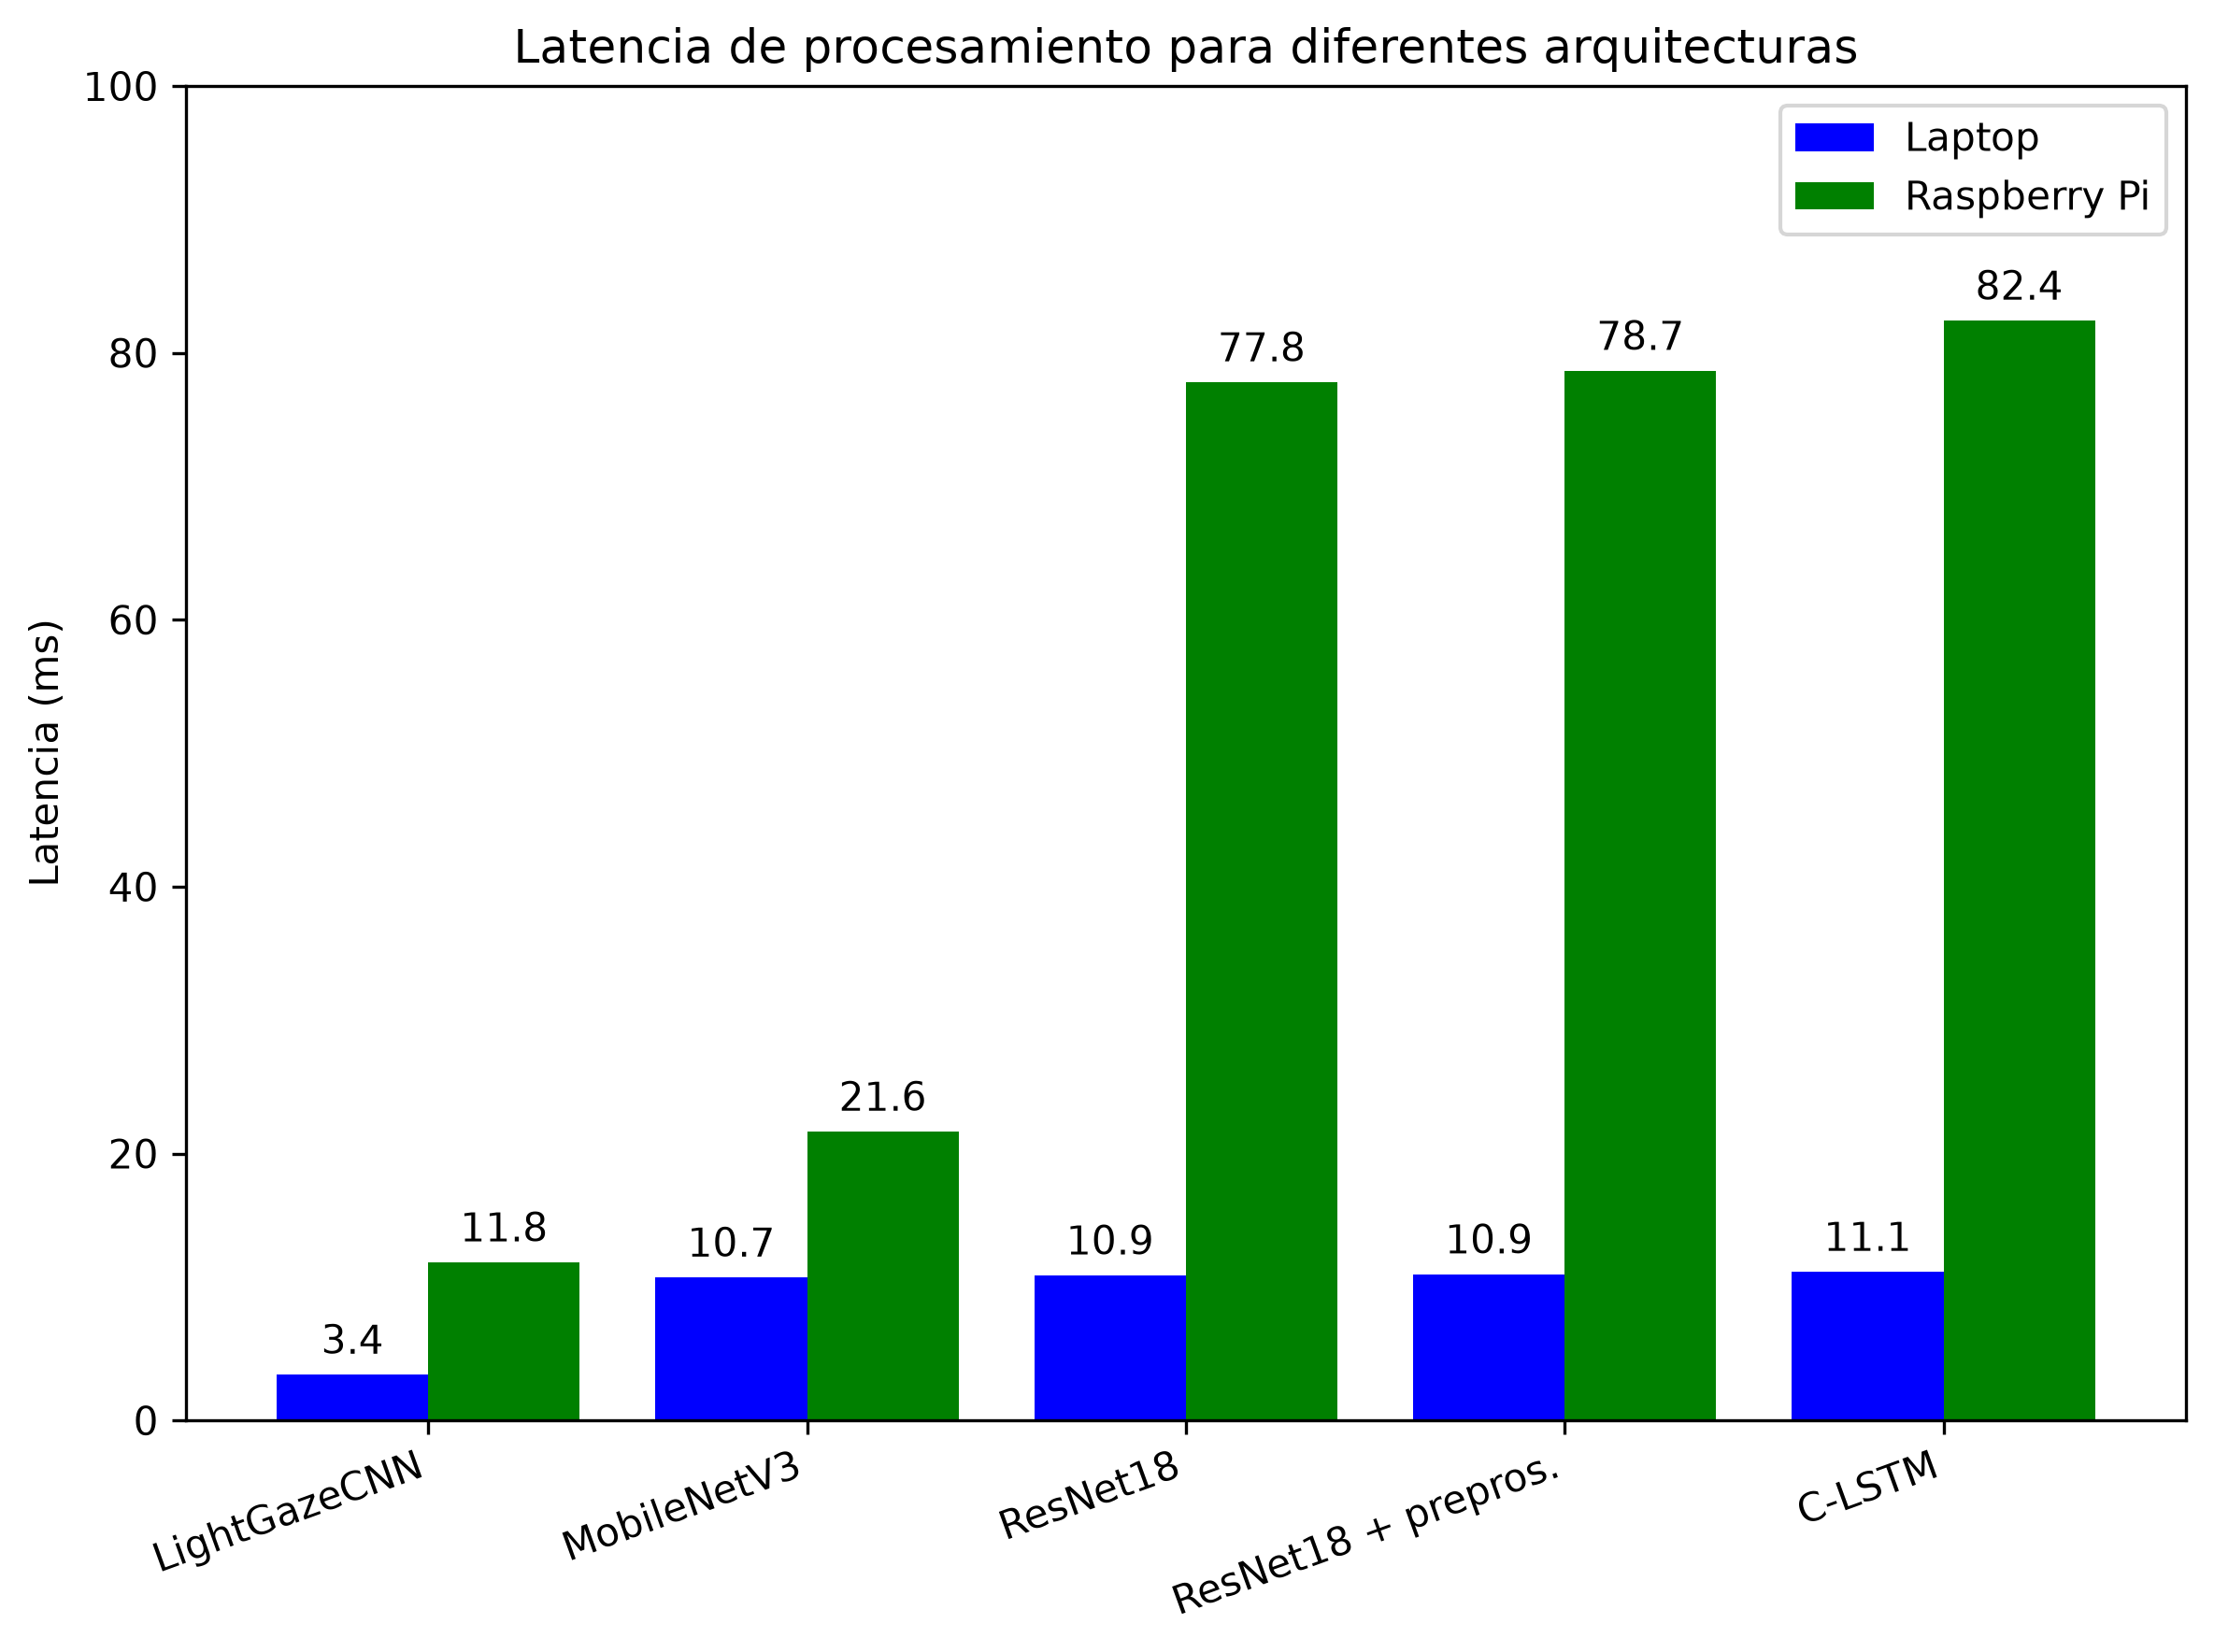
\includegraphics[width=0.6\linewidth]{figures/latencia_arquitecturas.png}
    \caption{Resultados de experimentación en entrenamiento de modelos de aprendizaje profundo}
    \label{fig:lat}
\end{figure}


\section{Detección de somnolencia}
\subsection{Detección de parpadeo y PERCLOS}
\subsection{Detección de bostezo}
\subsection{Cálculo de orientación de cabeza}
Para determinar si los resultados del algoritmo de cálculo de orientación de cabeza son óptimos, se compararon las métricas obtenidas en el análisis con el conjunto de datos \textit{Head Tracking} de la Universidad de Boston con las presentadas en la investigación de Choi y Kim, que utilizan este mismo conjunto de datos para su análisis. La Figura \ref{fig:HeadPose} muestra esta comparativa, la barra azul mostrando los valores de MAE obtenidos por nuestro algoritmo, y la barra roja representando los valores obtenidos por Choi y Kim.

\begin{figure}[h!]
    \centering
    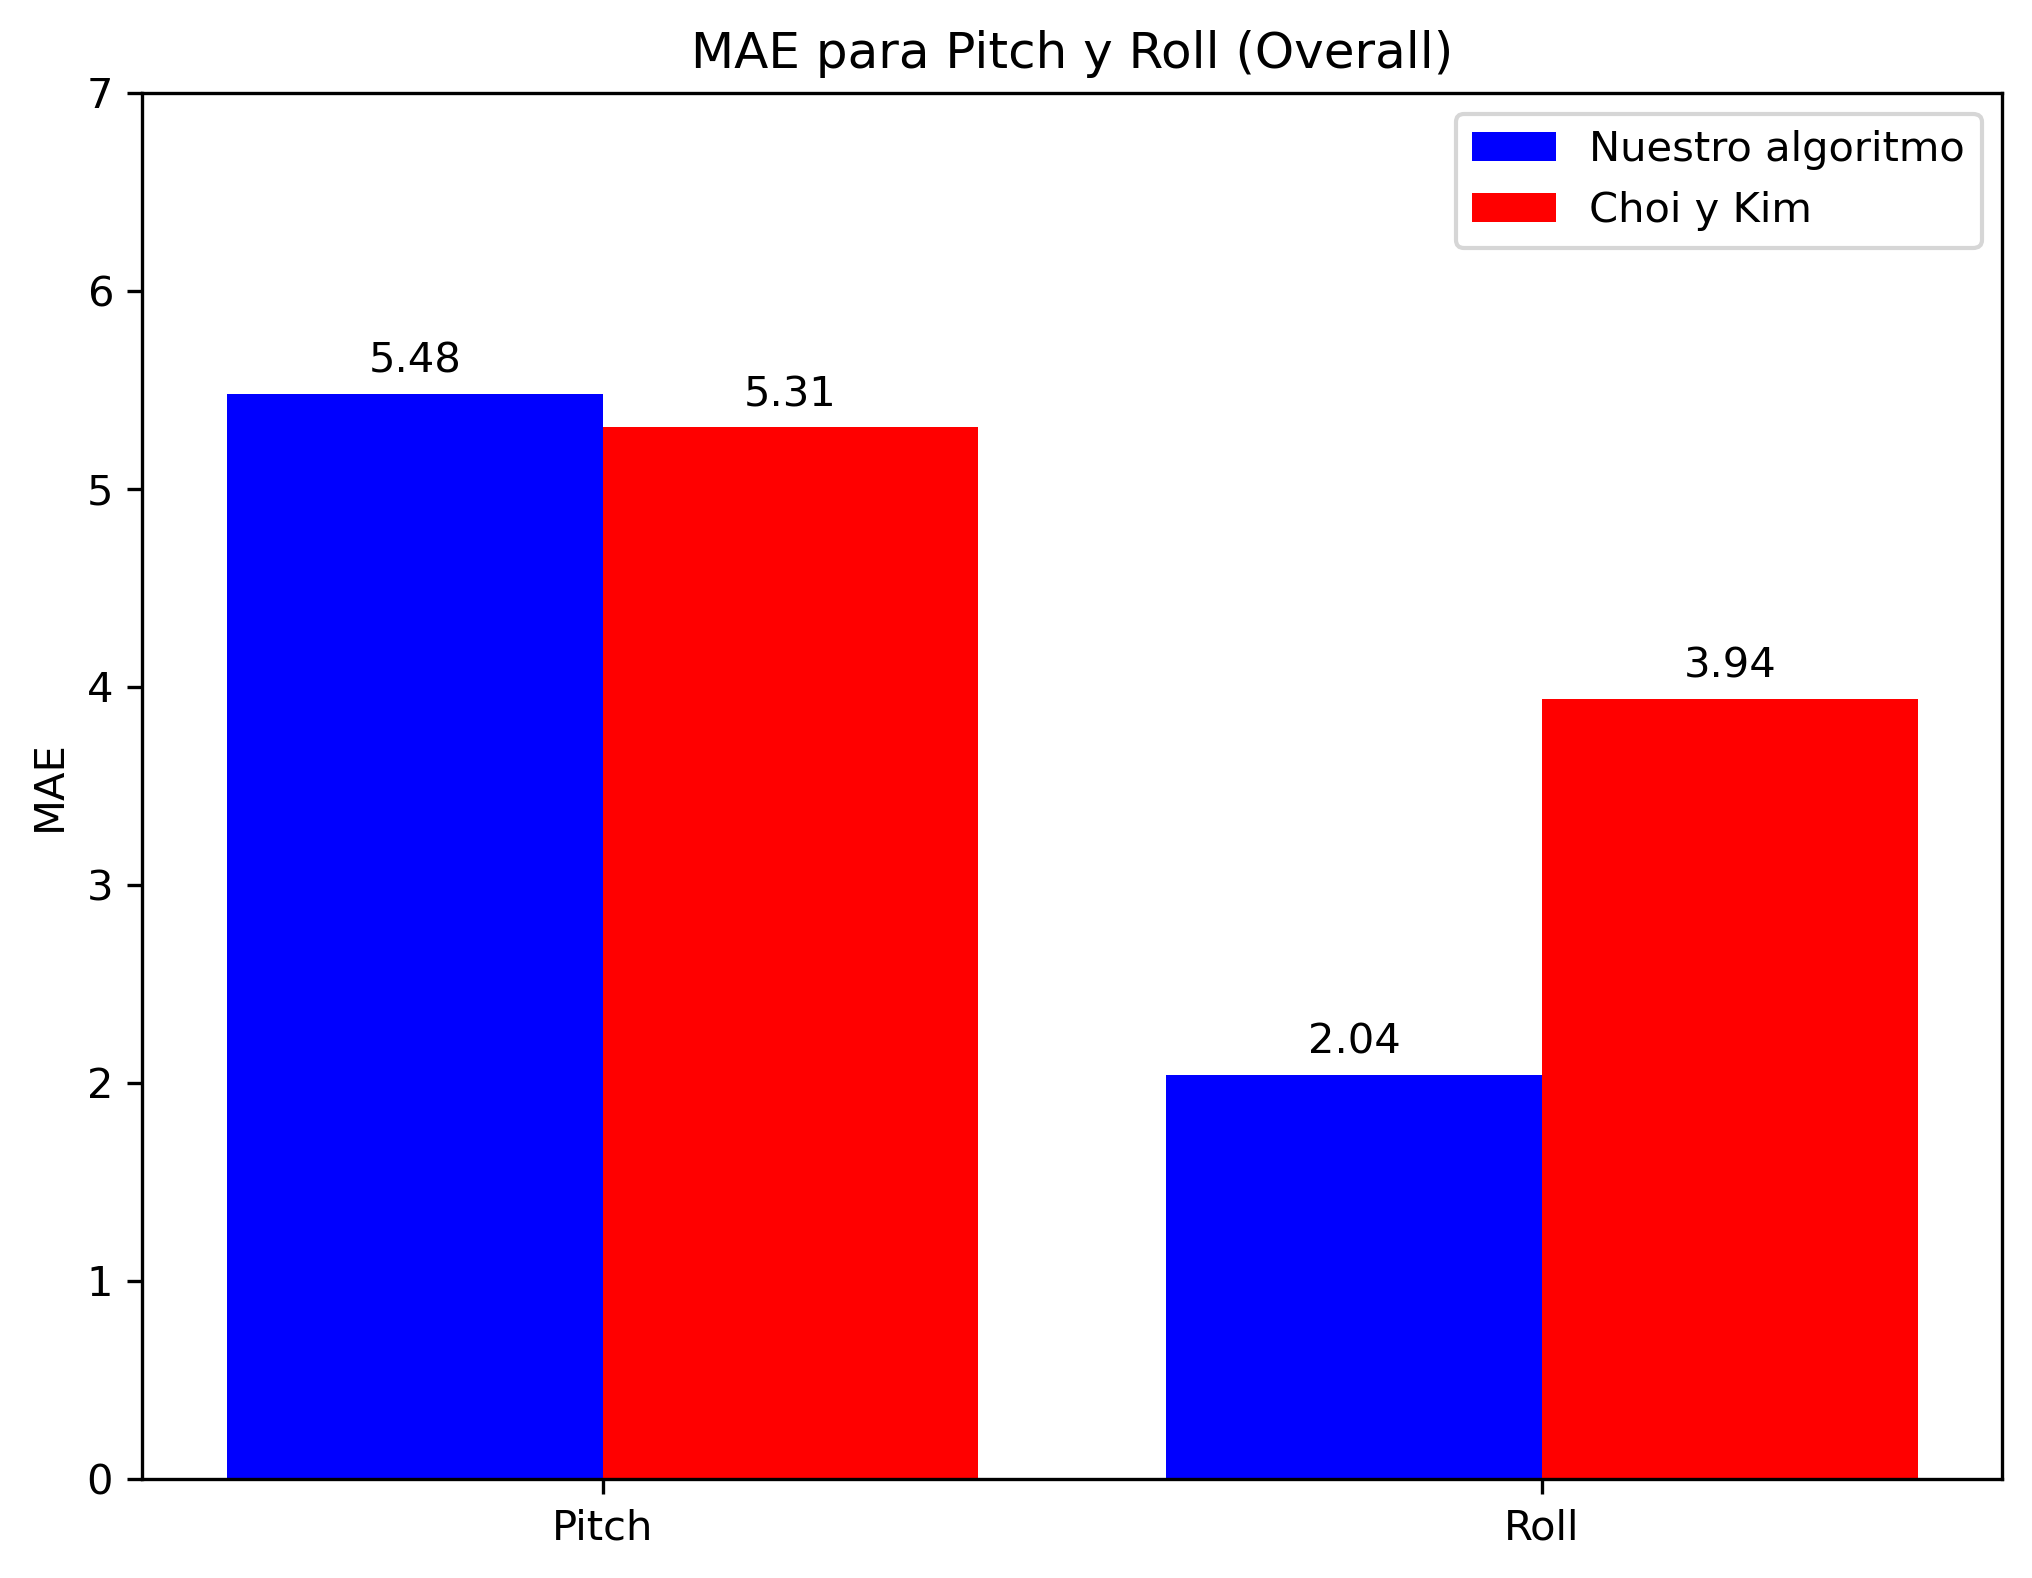
\includegraphics[width=0.7\linewidth]{figures/MAE_Overall.png}
    \caption{Comparativa de métricas resultantes de algoritmos de orientación de cabeza}
    \label{fig:HeadPose}
\end{figure}

\newpage %por ahora
\section{Resultados de codigo modular en tiempo real}
Se realizaron pruebas de funcionamiento del código modular en tiempo real, utilizando la RaspberryPi 5B como dispositivo de prueba. 
Esto se realizó para la versión modular en Python y en  C++, con el objetivo de observar la mejora en eficiencia al cambiar de Python a C++, 
vez se determino que el lenguaje de Python era muy lento para ser implementado en tiempo real. Ambas pruebas se realizaron utilizando la C-LSTM como arquitectura para la detección de distracción, buscando comparar ambos lenguajes en el caso más demandante del algoritmo. 

La Tabla \ref{tab:Python} muestra los resultados de latencia promedio obtenidos en la versión modular en Python. La detección de somnolencia, que incluye la detección de rostro, los 68 puntos, y el cálculo de PERCLOS, duración de parpadeo, orientación de cabeza y detección de bostezo, tiene una duración de 44.65ms. Donde vemos una latencia grande, como ya se observo en los resultados individuales, es en la detección de distracción, que tarda en promedio 79.87ms en realizarse cuando se utiliza una C-LSTM para realizar la predicción. Aunque este es un resultado ligeramente mejor que los inicialmente obtenidos, este sigue siendo muy tardado, generando que le algoritmo en tiempo real alcance tan solo 7.7 FPS en promedio, muy por debajo del objetivo. 

\begin{table}[h!]
    \centering
    \footnotesize
    \begin{tabular}{c c}
        Tarea & Latencia (ms) \\
        \hline
        Detección de somnolencia & 44.65 \\
        Detección de distracción & 79.87 \\ 
        \hline
    \end{tabular}
    \caption{Tiempos de latencia en codigo modular de Python}
    \label{tab:Python}
\end{table}

En la Tabla \ref{tab:C} se observan las latencias promedio obtenidas en la versión final del código modular en C++. El valor de la tarea de somnolencia es de 54.85ms, tomando en cuenta la implementación de la detección de rostro, cálculo de PERCLOS, duración de parpadeo, orientación de cabeza, y detección de bostezo a través de una CNN. La detección de distracción, que cumple con las mismas tareas que en Python, tiene una latencia promedio de 77ms. Se destaca que debido a que esta versión utiliza \textit{threading}, los timepos de inferencia de cada tarea no se suman, si no que suceden a diferente velocidad en paralelo. Al observar el funcionamiento de este algoritmo en tiempo real, se obtienen FPS de 13 y 18.89 para las tareas de distracción y somnolencia, respectivamente. Esta velocidad es la necesaria para que se presente un funcionamiento en tiempo real correcto y fluido.
\begin{table}[h!]
    \centering
    \footnotesize
    \renewcommand{\arraystretch}{1.8} 
    \begin{tabular}{c c}
        Tarea & Latencia (ms) \\
        \hline
        Detección de somnolencia & 54.85 \\
        Detección de distracción & 77.00 \\ 
        \hline
    \end{tabular}
    \caption{Tiempos de latencia en codigo modular de C++}
    \label{tab:C}
\end{table}

La Figura \ref{fig:grouped} ilustra los distintos estados que se pueden encontrar en el código modular de C++. Existe el estado de condición segura, el estado de distracción y el estado de somnolencia. También puede apreciarse la funcionalidad de las métricas secundarias, el bostezo y la orientación de la cabeza, donde puede suceder que se detecten pero no se marque un estado de somnolencia ya que no se cumplen con los requisitos para indicar alarma.  

\begin{figure}[h!]
    \centering
    % Row 1: 2 images
    \begin{minipage}{0.45\textwidth}
        \centering
        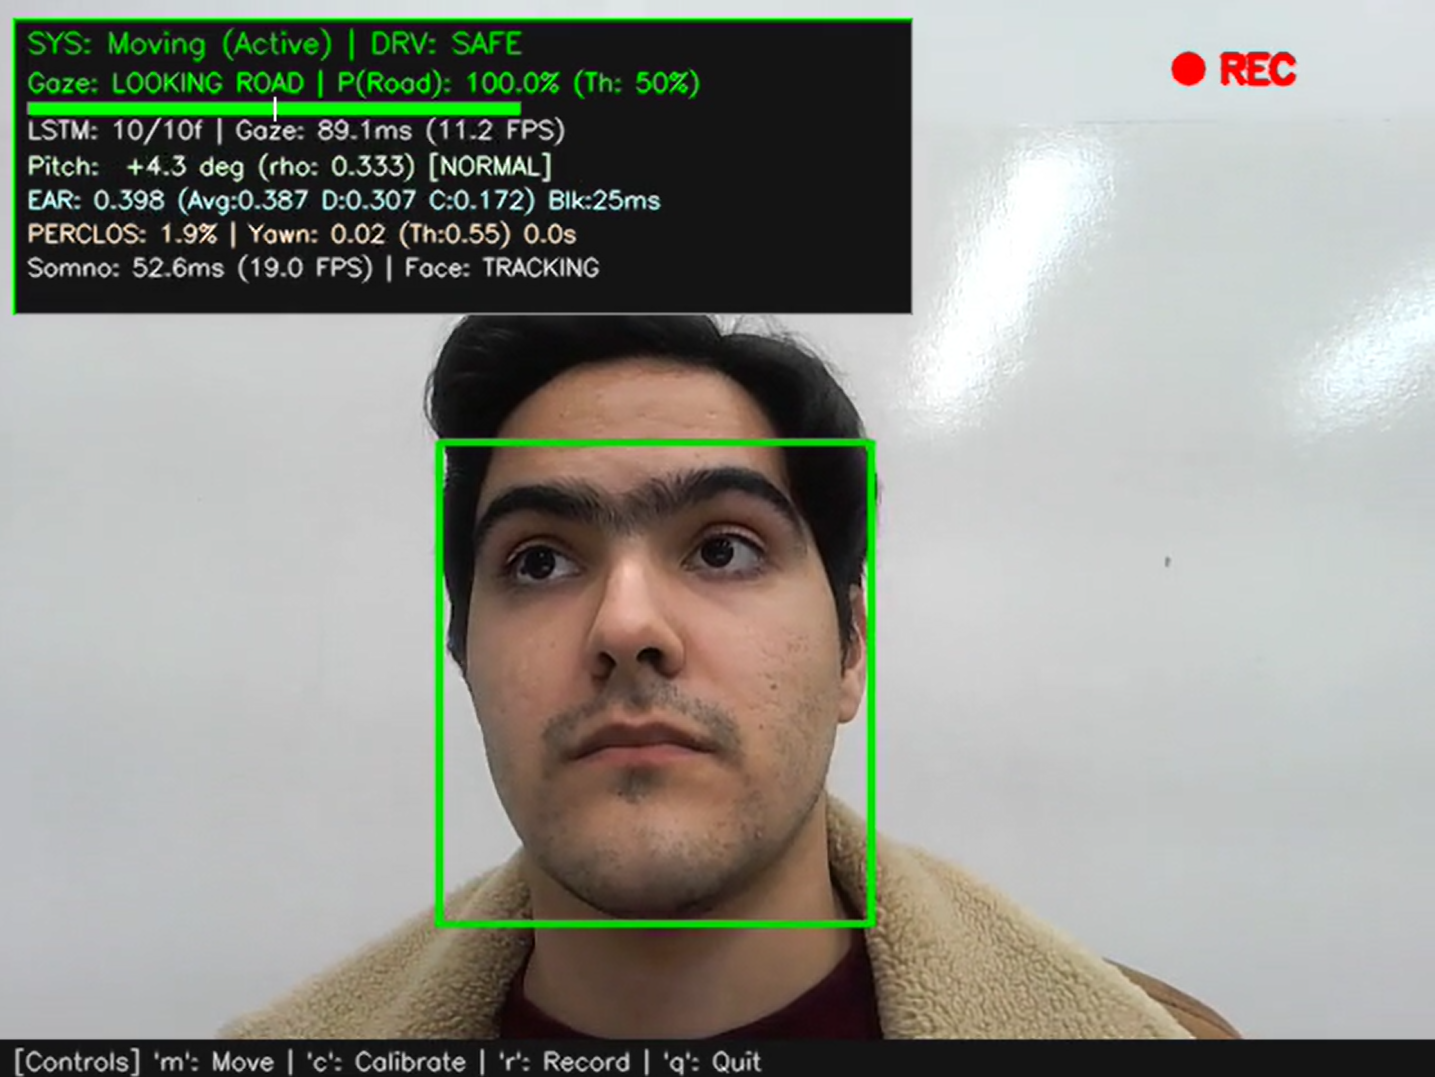
\includegraphics[width=\textwidth]{figures/imagen muestra dem.png}
    \end{minipage}\hfill%
    \begin{minipage}{0.45\textwidth}
        \centering
        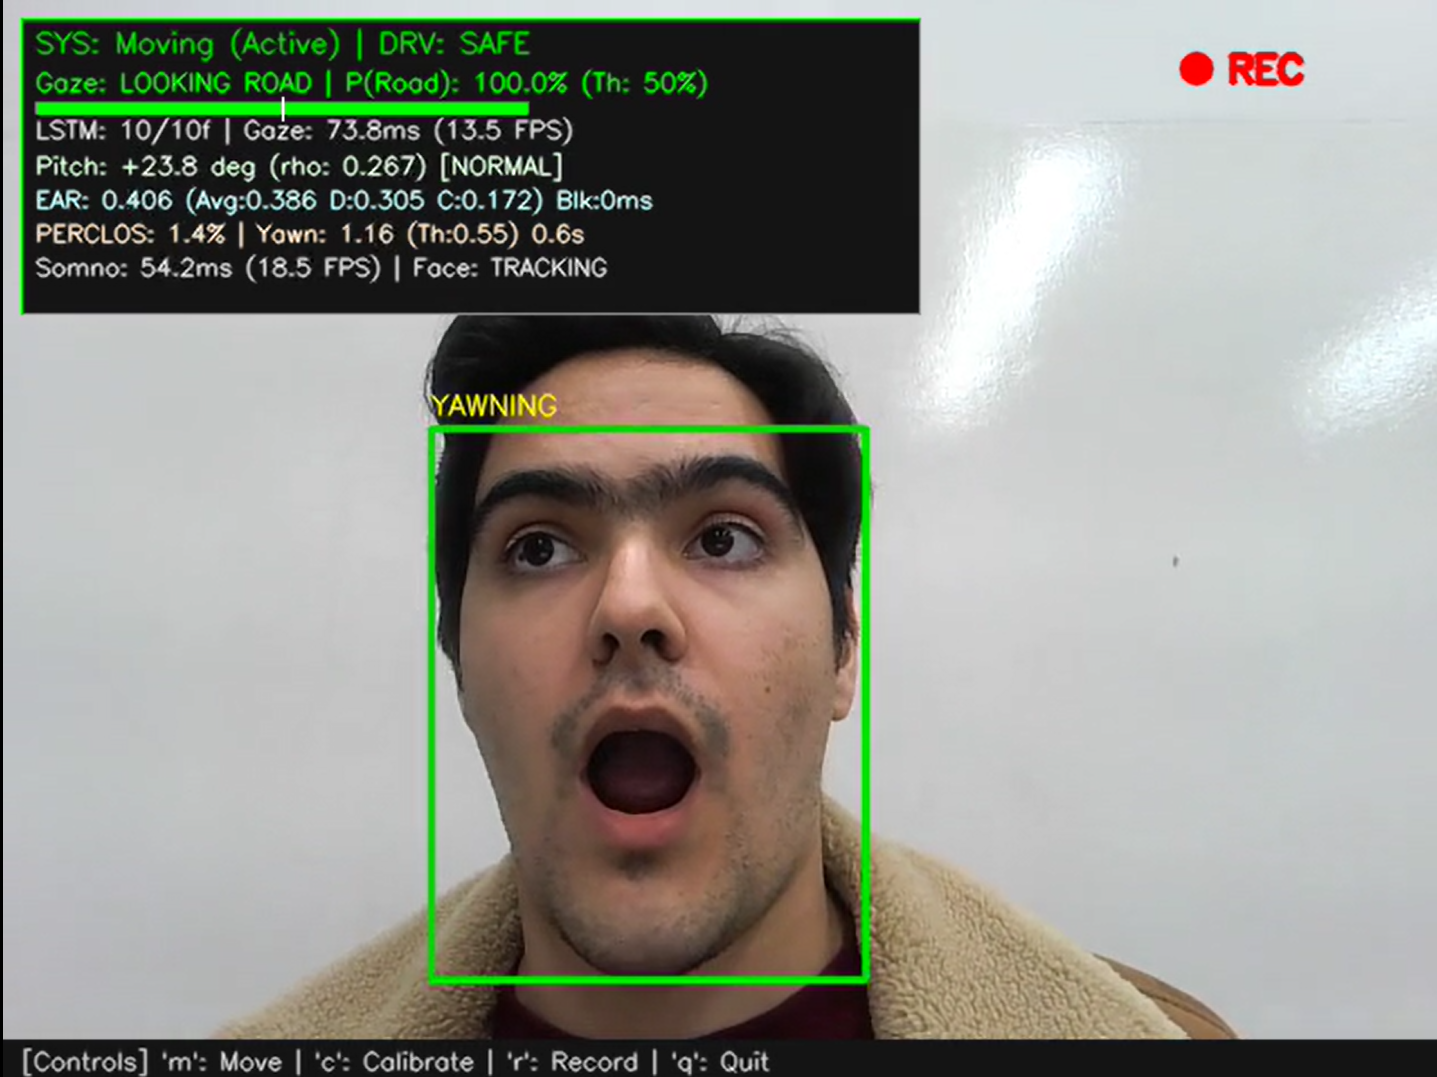
\includegraphics[width=\textwidth]{figures/imgyawn.png}
    \end{minipage}

    \vspace{0.3cm}

    % Row 2: 2 images
    \begin{minipage}{0.45\textwidth}
        \centering
        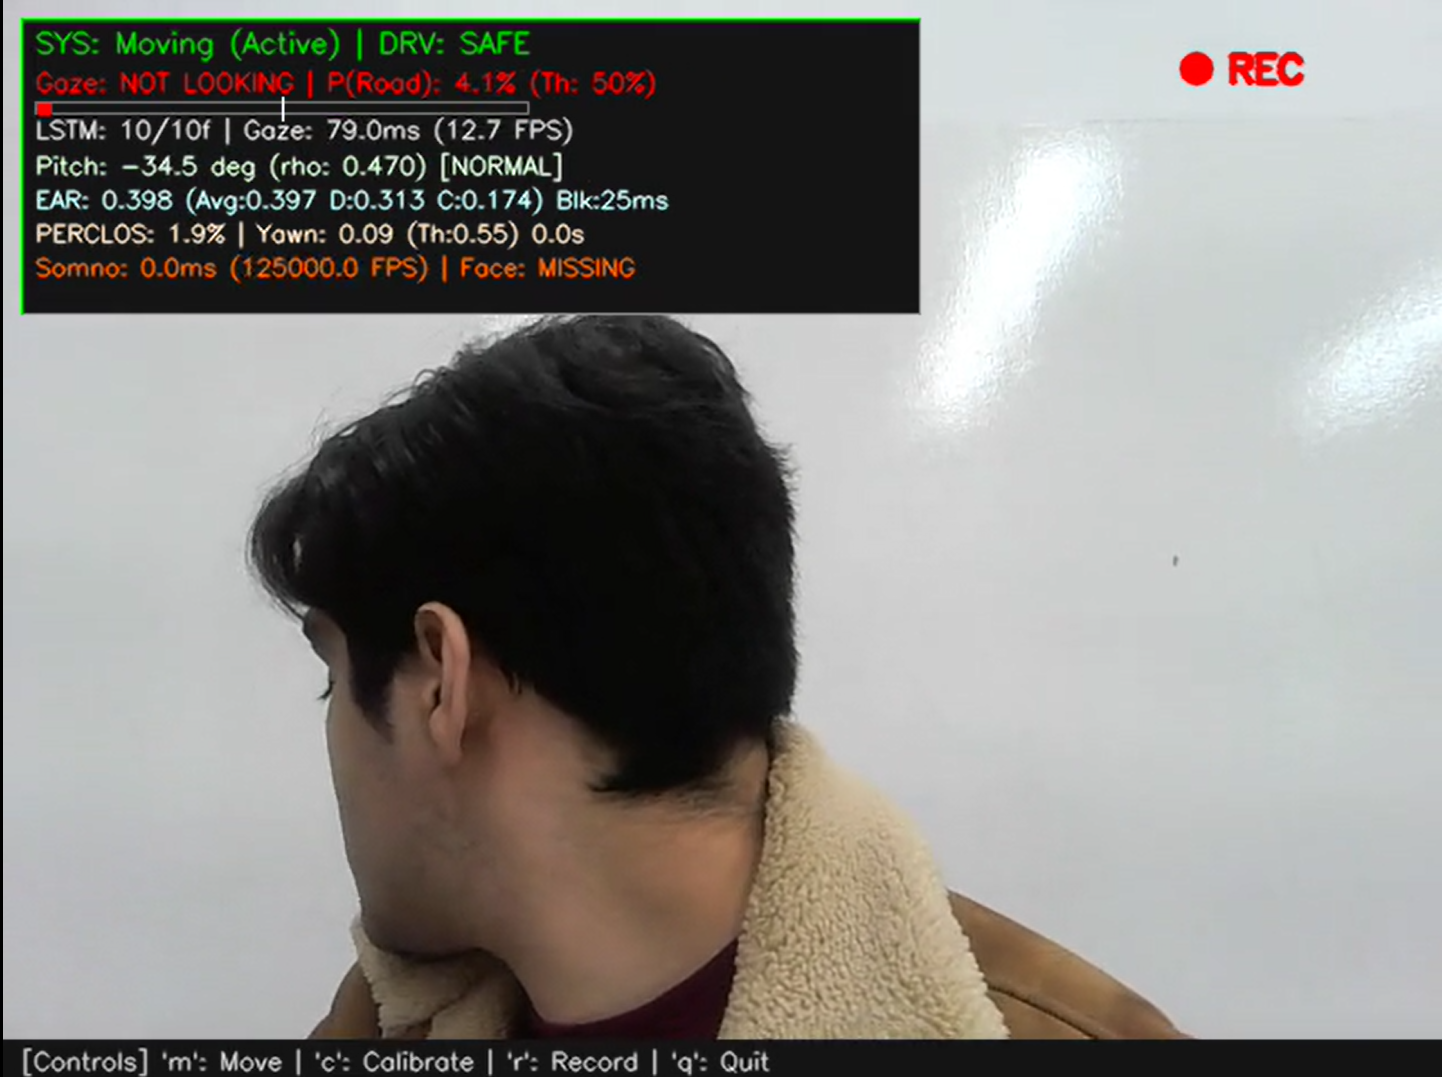
\includegraphics[width=\textwidth]{figures/imgdist.png}
    \end{minipage}\hfill%
    \begin{minipage}{0.45\textwidth}
        \centering
        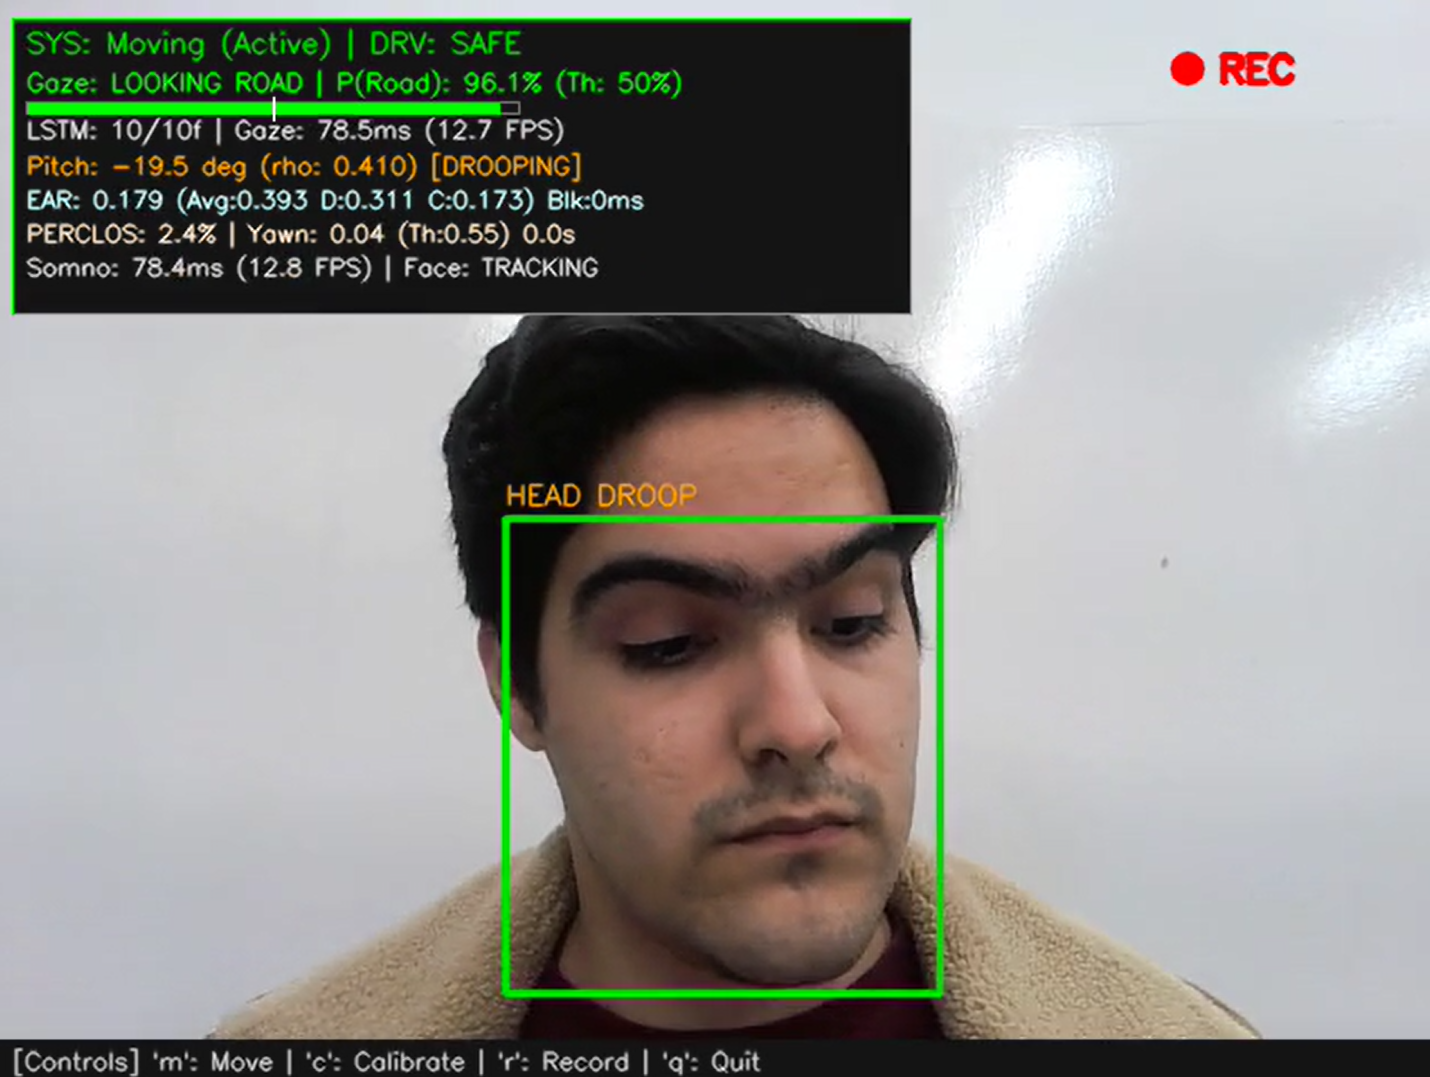
\includegraphics[width=\textwidth]{figures/imghead.png}
    \end{minipage}

    \vspace{0.3cm}

    % Row 3: 1 image
    \begin{minipage}{0.45\textwidth}
        \centering
        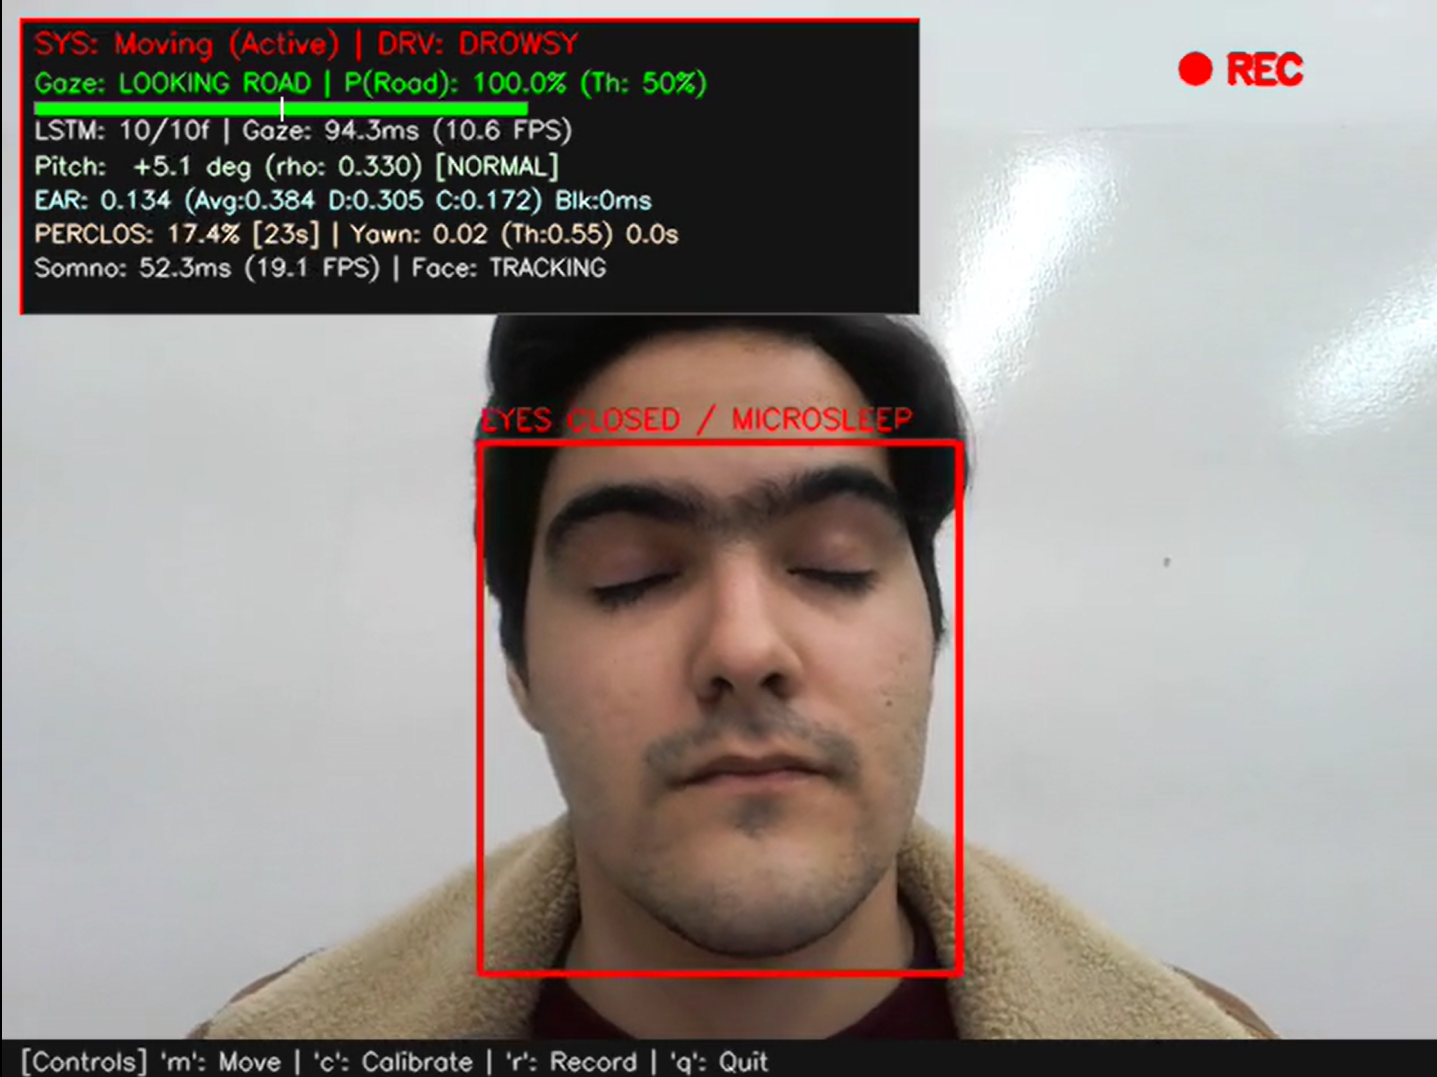
\includegraphics[width=\textwidth]{figures/imgparp.png}
    \end{minipage}

    \caption{Imágenes ilustrativas de distintos estados del código mostrados en debug}
    \label{fig:grouped}
\end{figure}